\documentclass[preview]{standalone}
%\usepackage[active,tightpage]{preview}
%\PreviewBorder=12pt

\usepackage{tikz}
\usetikzlibrary{decorations.pathmorphing,patterns,calc,positioning}

\begin{document}
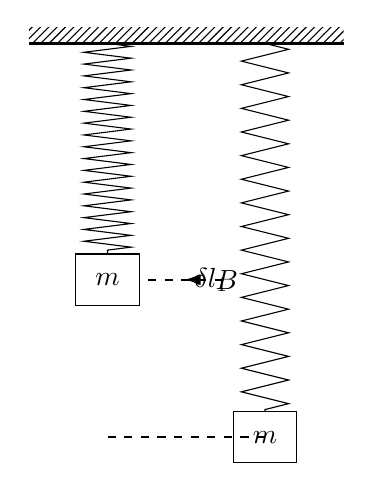
\begin{tikzpicture}
\node[rectangle,draw=black,inner sep=2.5mm] (a) at (0,2) {$m$};
\node[rectangle,draw=black,inner sep=2.5mm] (b) at (2,0) {$m$};
\draw[decoration={aspect=0.3, segment length=1.5mm, amplitude=3mm,zigzag},decorate] (0,5) -- (a); 
\draw[decoration={aspect=0.3, segment length=3mm, amplitude=3mm,zigzag},decorate] (2,5) -- (b); 
\fill [pattern = north east lines] (-1,5) rectangle (3,5.2);
\draw[thick] (-1,5) -- (3,5);

\begin{scope}
%\myfig{2mm}{-4.8cm}{-0.35cm}{1.5}
\node[draw=none,right=.25cm] at (1,2)(b) {$B$};
\draw [thick,dashed] ($(b) + (-1,0)$) -- +(1,0)node[draw=none,inner sep = 0,pos=.5](b1){};
\draw[thick,latex-latex] ($(a) + (1,0)$) -- (b1)node[draw=none,inner sep = 0,pos=.5,right=0.1cm]{$\delta l_1$};
\draw[thick,dashed] (0,0) -- +(2,0)node[draw=none,inner sep = 0,pos=.5]{};
\end{scope}

\end{tikzpicture}
\end{document}